\section{A Solvable Theoretical Setting}

\label{app:th_rf}


The agnostic and recursive nature of Neural LoFi calls for a theoretical setting that contains a compositional structure, while not revealing the relevant intermediate variables to the learner. In this appendix, we follow the hierarchical spectral construction of \cite{tabanelli2026deep}, building on the fundamental  earlier works \cite{wang2024learning,nichani2023provable,fu2025learning}. 
This allows us to define a controlled high-dimensional model and to use it to study how depth turns a globally hard learning problem into a sequence of simpler spectral recoveries.

A natural way to isolate the role of depth is to consider teacher-student models where the target is not merely a low-dimensional function of the input, but is built through a hierarchy of intermediate representations. Such models have appeared in several recent works on compositional learning and the computational advantage of depth, including random hierarchy models, hierarchical Gaussian targets, and polynomial teacher-student constructions (e.g.
\cite{cagnetta2024how,garnierbrun2025how,dandi2026computational,wang2024learning,nichani2023provable,fu2025learning,cagnetta2025learning,tabanelli2026deep,cagnetta2026deriving,ren2026provable}). 
They share the same guiding principle: a target may look high-dimensional or high-degree as a function of the input, while becoming low-degree after the right intermediate representation has been found. This is precisely the situation in which depth should help, since learning can proceed by a sequence of simpler feature-recovery problems rather than by solving the full high-degree task at once.

\subsection{Setting}\label{subsec:set_th}

We focus on the high-dimensional Gaussian teacher-student model of \cite{tabanelli2026deep}, which provides a particularly tractable instance of this principle. The input is Gaussian, $\bx\sim\mathcal N(0,I_d)$, and the target is generated by a two-level compositional hierarchy
\begin{align}
    \bx \in \mathbb R^d
    \quad \longrightarrow \quad
    h^{(1)}(\bx) \in \mathbb R^{d_1}
    \quad \longrightarrow \quad
    h^{(2)}(\bx) \in \mathbb R
    \quad \longrightarrow \quad
    y .
\end{align}
For $q\geq 1$, we denote by $H_q(\cdot)$ the normalized Hermite polynomial of order $q$, either in its scalar or tensor-valued form.\footnote{
For a vector $\bx\in\mathbb R^m$, the tensor Hermite polynomial $H_q(\bx)\in(\mathbb R^m)_{\mathrm{sym}}^{\otimes q}$ is defined through the tensorial Rodrigues formula
$
\sqrt{q!}\,H_q(\bx)
=
(-1)^q e^{\|\bx\|^2/2}
\nabla_{\bx}^{\otimes q}
\left(e^{-\|\bx\|^2/2}\right),
$
where $\nabla_{\bx}^{\otimes q}$ denotes the $q$-fold symmetric tensor of derivatives. 
For $m=1$, this reduces to the normalized scalar Hermite polynomial
$
\sqrt{q!}\,H_q(z)
=
(-1)^q e^{z^2/2}
\frac{d^q}{dz^q}
\left(e^{-z^2/2}\right).
$
}
We write $\langle\cdot,\cdot\rangle$ for the Frobenius product between tensors of the same order.\footnote{
For example, if $\bx\in\mathbb R^m$ and $A\in\mathbb R^{m\times m}$ is symmetric, then
$
\left\langle A,H_2(\bx)\right\rangle
=
\frac{1}{\sqrt{2}}
\left(
    \bx^\top A\bx-\mathrm{Tr}(A)
\right).
$
}
We write $F_q$ for the symmetric flattening map from order-$q$ symmetric tensors to $\mathbb R^{D_q}$, with $D_q=\binom{d+q-1}{q}$, chosen so that the Frobenius product is preserved. 
Below, we freely identify a symmetric tensor with its flattened representation whenever no ambiguity arises. The teacher parameters are given by symmetric tensors
\begin{align}
    A_i^{(1)}
    \in
    (\mathbb R^d)_{\mathrm{sym}}^{\otimes q},
    \qquad
    i=1,\ldots,d_1,
    \qquad
    d_1=d^\epsilon,
\end{align}
normalized so that the first-layer features have order-one variance, and by a symmetric matrix
\begin{align}
    A^{(2)}
    \in
    \mathbb R^{d_1\times d_1}.
\end{align}
The latent variables and the label are then defined as
\begin{align}
    h^{(1)}_i(\bx)
    &=
    \left\langle
        A_i^{(1)}, H_q(\bx)
    \right\rangle,
    \qquad i=1,\ldots,d_1, \\
    h^{(2)}(\bx)
    &=
    \left\langle
        A^{(2)}, H_2(h^{(1)}(\bx))
    \right\rangle, \\
    y
    &=
    g^\star(h^{(2)}(\bx)).
\end{align}
Thus the first layer selects only $d_1=d^\epsilon$ directions inside the ambient degree-$q$ Hermite space of dimension $D_q$. When $d_1\ll D_q$, the relevant information is sparse in this low-degree feature space: the target depends on $\bx$ only through a small hidden subspace of Hermite features. Learning the first layer therefore amounts to recovering this subspace, so that the rest of the hierarchy can be expressed as a low-degree problem in the variables $h^{(1)}$.

The analysis of \cite{tabanelli2026deep} shows that this sparse compositional structure can be exploited by a hierarchical spectral estimator. Rather than learning the full composed function in one step, the procedure first recovers the hidden degree-$q$ subspace defining $h^{(1)}$, and then uses this recovered representation to make the next component of the hierarchy accessible. In this sense, depth turns the learning problem into a sequence of spectral recovery tasks, each one exposing the variables needed by the next layer.

This gives a clean explanation for the advantage of depth in this model. A one-shot method that works directly on the input must resolve the full high-degree dependence of $y$ on $x$. By contrast, the hierarchical spectral procedure only needs to reveal the first representation and then reuse it to make the next layer visible. In the regime $d_1=d^\epsilon$, the first stage requires on the order of $d^{q+\epsilon}$ samples, while the second stage requires only the sample complexity of a quadratic problem in dimension $d_1$. The dominant cost is therefore the recovery of the first hidden representation, rather than the degree of the full composed polynomial.

The price to pay is that the corresponding spectral estimators are still partially co-designed with the Gaussian-Hermite structure of the teacher. Indeed, the first stage is built in an explicit degree-$k$ Hermite feature space, while the second stage uses a prescribed second-order Hermite structure in the recovered variables. A natural way to relax this feature-design aspect is to replace the explicit Hermite construction by nonlinear random features. Rather than specifying the polynomial coordinates in advance, one lets a random feature map generate a generic nonlinear representation and applies the same layer-wise spectral selection in that space. In the hierarchical teacher-student setting above, this random-feature extension of the hierarchical spectral estimator matches precisely the Neural LoFi algorithm.

\subsection{Random-feature hierarchical estimator}
\label{app:rf-estimator}

In this setting, Neural LoFi takes the following concrete form. Let $W_1=(w_{1,a})_{a=1}^{p_1}$ with $w_{1,a}\sim \mathrm{Unif}(\mathbb S^{d-1})$, and define the first random-feature representation
\begin{align}
    \phi^{(1)}_\mu
    =
    \frac{1}{\sqrt{p_1}}
    \sigma_1(W_1 x_\mu)
    \in \mathbb R^{p_1}.
\end{align}
The first spectral operator is
\begin{align}
    \widehat C_1
    =
    \frac1n
    \sum_{\mu=1}^n
    y_\mu
    \phi^{(1)}_\mu
    \phi^{(1)\top}_\mu .
\end{align}
Let $\widehat V_1\in\mathbb R^{p_1\times d_1}$ contain the eigenvectors of $\widehat C_1$ associated with the largest eigenvalues in absolute value. Here we keep $d_1$ directions for simplicity; this can be replaced by a standard rank-selection step. The recovered first-layer coordinates are
\begin{align}
    \widehat h^{(1)}_\mu
    =
    \widehat V_1^\top \phi^{(1)}_\mu
    \in \mathbb R^{d_1}.
\end{align}
We then draw $W_2=(w_{2,a})_{a=1}^{p_2}$ with $w_{2,a}\sim \mathrm{Unif}(\mathbb S^{d_1-1})$, and define
\begin{align}
    \phi^{(2)}_\mu
    =
    \frac{1}{\sqrt{p_2}}
    \sigma_2(W_2 \widehat h^{(1)}_\mu)
    \in \mathbb R^{p_2}.
\end{align}
At the second layer, since the teacher contains only one hidden direction, we do not construct a matrix-valued spectral estimator. Instead, we directly form the first-order moment vector
\begin{align}
    \widehat v_2
    =
    \frac1n
    \sum_{\mu=1}^n
    y_\mu
    \phi^{(2)}_\mu .
\end{align}
The associated second-layer coordinate is then obtained by projection:
\begin{align}
    \widehat h^{(2)}_\mu
    =
    \widehat v_2^\top \phi^{(2)}_\mu .
\end{align}
Finally, the readout is fitted on the one-dimensional representation $\{(\widehat h^{(2)}_\mu,y_\mu)\}_{\mu=1}^n$, for instance by ridge regression in a polynomial feature space,
\begin{align}
    \widehat g
    \in
    \arg\min_{g\in\mathcal G}
    \frac1n
    \sum_{\mu=1}^n
    \left(
        y_\mu - g(\widehat h^{(2)}_\mu)
    \right)^2
    +
    \lambda \|g\|_{\mathcal G}^2 .
\end{align}

The choice of keeping exactly \(d_1\) eigenvectors at the first layer is not meant to define a different procedure, but simply to make explicit the outcome of the usual rank-selection step within Neural LoFi in the present setting. More generally, one could keep an arbitrary number \(k\) of directions and optimize over \(k\), exactly as in the rest of the pipeline. In the model considered here, this optimization would select \(d_1\) directions at the first layer and a single direction at the second layer. In that sense, fixing \(d_1\) in the first layer and using the linear estimator \(\widehat v_2\) in the second layer is fully equivalent to the standard Neural LoFi selection rule.


\subsection{Main Results}\label{subsec:th_main_results}

The main prediction of this tractable model is that replacing the explicit Hermite structure of the estimator by random features preserves the emergence transition. In particular, for a degree-$q$ first layer with $d_1=d^\epsilon$ hidden variables, we expect the first representation $h^{(1)}$ to become recoverable at the sample scale
\begin{align}
    n
    \gg
    d^{q+\epsilon}.
\end{align}
In the quadratic setting used in our experiments, $q=2$, and the predicted first-stage transition is therefore $n \gg d^{2+\epsilon}$.

This prediction is the concrete instance of the emergence criterion in Eq.~\eqref{eq:emergence_feature} in the main text. Indeed, Eq.~\eqref{eq:emergence_feature} states that the empirical fluctuation level is governed by the effective dimension of the current residual feature class. Section~\ref{app:effective-dimension-hermite} shows that, before the first hidden variables have been recovered, the relevant effective dimension is the size of the degree-$q$ Hermite block, namely $D_q=O(d^q)$. The additional factor $d_1=d^\epsilon$ comes from separating and aligning with the $d_1$ planted directions in this block, giving the scale $D_qd_1=O(d^{q+\epsilon})$.

The role of the next subsection is to explain why the random-feature estimator contains the same signal-bearing Hermite spectral object as the explicit construction, now embedded in the random-feature representation. Figure~\ref{fig:rf_theoretical} illustrates the resulting transition numerically: in the quadratic case, the drop in MSE, the growth of the overlap with $h^{(1)}$, and the separation of the leading eigenvalues all occur at the predicted first-layer emergence scale.



\subsection{Mathematical Justification}\label{gif:rf_maths}

We now analyze the signal structure of the random-feature estimator introduced above. The key point is that, although the estimator is built from generic nonlinear random features, its population signal behaves as a well-defined Hermite estimator aligned with the teacher hierarchy. This will allow us to connect the first step of the Neural LoFi algorithm to the spectral transition established in the Hermite model of \cite{tabanelli2026deep}.

Let us expand the first-layer activation in Hermite as
\begin{align}
    \sigma_1(z)
    =
    \sum_{q\geq 2}
    c_q H_q(z),
    \qquad
    c_q
    =
    \mathbb E_{z\sim \mathcal N(0,1)}
    \left[
        \sigma_1(z)H_q(z)
    \right],
\end{align}
where $H_q$ denotes the normalized scalar Hermite polynomial of degree $q$.
For each row $\bw_{1,a}$ of $W_1$, we use the standard Hermite tensor identity
\begin{align}
    H_q(\langle \bw_{1,a},\bx\rangle)
    =
    \left\langle
        \bw_{1,a}^{\otimes q},
        H_q(\bx)
    \right\rangle .
\end{align}
Here and below, $\bw_{1,a}^{\otimes q}$ denotes the degree-$q$ Hermite coefficient vector, with the multi-index normalization chosen so that the above identity holds. Collecting these coefficient tensors over all rows of $W_1$, and flattening them with the Frobenius-preserving map $F[\cdot]$, we define:
\begin{align}
    \frac{1}{\sqrt{p_1}} H_q(W_1\bx)
    =
    P_q H_q(\bx),\quad \textrm{with} \quad P_q
    :=
    \frac1{\sqrt{p_1}}
    \begin{bmatrix}
        F[\bw_{1,1}^{\otimes q}]^\top \\
        \vdots \\
        F[\bw_{1,p_1}^{\otimes q}]^\top
    \end{bmatrix}
    \in \mathbb R^{p_1\times D_q}.
\end{align}
where $H_q(W_1\bx)\in\R^{p_1}$ is understood entrywise on the left-hand side and $H_q(\bx)\in \R^{D_q}$ is the flattened Hermite tensor. Hence the first random-feature representation decomposes as
\begin{align}
    \phi_\mu^{(1)}
    =
    \frac{1}{\sqrt{p_1}}\sigma_1(W_1\bx_\mu)
    =
    \sum_{q\geq 2}
    c_q
    P_q H_q(\bx_\mu).
\end{align}

We denote by
\begin{align}
    \widehat C_H^{(q)}
    :=
    \frac1n
    \sum_{\mu=1}^n
    y_\mu
    H_q(\bx_\mu)H_q(\bx_\mu)^\top
\end{align}
the degree-$q$ Hermite moment matrix appearing in the middle. If one uses the centered second-order Hermite convention of \cite{tabanelli2026deep}, this matrix should be replaced by its centered version; the difference is an empirical isotropic term, controlled by the same estimates and absorbed in the rates below. With this notation, the degree-$q$ contribution to
the first Neural LoFi operator is
\begin{align}
    \widehat C_{\rm RF}^{(q)}
    =
    c_q^2
    P_q
    \widehat C_H^{(q)}
    P_q^\top .
\end{align}
Thus the random-feature operator contains the Hermite estimator conjugated by the random
Hermite embedding $P_q$, up to the scalar factor $c_q^2$.

We now focus on the quadratic case $q=2$, which is the case controlled explicitly by the quadratic Hermite decomposition of \cite{wen2025when}. Define the normalized RF Gram
\begin{align}
    G_2
    :=
    D_2 P_2^\top P_2 .
\end{align}
The important point is that $G_2$ is not close to the identity on the full degree-$2$ Hermite space. The trace direction produces a deterministic contraction spike. More precisely, by Lemma F.6 and Corollary F.7 of \cite{wen2025when}, one has the decomposition
\begin{align}
    G_2
    =
    I_{D_2}
    +
    K_2
    +
    R_2,
    \qquad
    K_2=\theta_d ee^\top,
    \qquad
    |\theta_d|\le \widetilde O(d),
\end{align}
where $e\in\mathbb R^{D_2}$ is the normalized trace direction in the degree-$2$ Hermite block. The term $K_2$ is the explicit non-trivial contraction term coming from the trace component of the quadratic Hermite features, while $R_2$ is the remaining centered fluctuation of the random-feature Gram, with
\begin{align}
    \|R_2\|_{\op}
    \le
    \widetilde O\!\left(
        \sqrt{\frac{D_2}{p_1}}
        +
        \frac{D_2}{p_1}
    \right),
\end{align}
where the $\widetilde O(\cdot)$ hides logarithmic factors in $d$. This conservative full-column concentration bound is not expected to be optimal, but it is sufficient for the projected comparison below.

Finally, let $A^{(1)}\in\mathbb R^{d_1\times D_2}$ be the matrix of planted first-layer Hermite directions, and define its random-feature image by
\begin{align}
    A_{\RF}^{(1)}
    :=
    \sqrt{D_2}\,
    A^{(1)}
    P_2^\top
    \in\mathbb R^{d_1\times p_1}.
\end{align}
% The normalization is chosen so that, on the planted subspace,
% $A_{\RF}^{(1)}$ has the same scale as $A^{(1)}$ whenever $G_2$ acts as the identity. 
We can now state the projected RF analogue of Theorem~3.1 in
\cite{tabanelli2026deep}.
\medskip

\begin{theorem}[Projected RF Hermite recovery, quadratic case]
\label{thm:rf-hermite-bridge-k2}
Assume the setting and normalization of Theorem~3.1 in
\cite{tabanelli2026deep}, with $d_1=d^\varepsilon$ and
$\varepsilon<1/2$. With $G_2$, $K_2$, $R_2$ as defined above, the following holds with
high probability:
\begin{align}
&\sqrt{d_1}
\left\|
    \frac{D_2}{c_2^2}
    A_{\RF}^{(1)}
    \widehat C_{\rm RF}^{(2)}
    A_{\RF}^{(1)\top}
    -
    \nu_1A^{(2)}
\right\|_{\op}
\nonumber\\
&\qquad\le
\widetilde O\!\left(
    \sqrt{\frac{d^2d_1}{n}}
\right)
+
\widetilde O\!\left(
    \frac{d_1}{\sqrt d}
\right)
+
\widetilde O\!\left(
    \frac1{\sqrt{d_1}}
\right)
\nonumber\\
&\qquad\quad+
\widetilde O\!\left(
    d_1\sqrt{\frac{d_1}{n}}
    +
    \frac{d_1^2}{d^2}
    +
    \sqrt{d_1} \left(
        \sqrt{\frac{D_2}{p_1}}
        +
        \frac{D_2}{p_1}
    \right)\left(1+
        \sqrt{\frac{D_2}{p_1}}
        +
        \frac{D_2}{p_1}
    \right)
\right).
\label{eq:rf-hermite-final-rate}
\end{align}
In particular, if
\[
    n\gg d^2d_1,
    \qquad
    p_1 \gg \sqrt{d_1}d^2,
\]
then the additional RF bridge error is $o(1)$. Therefore the projected RF
estimator has the same limiting signal as the Hermite estimator, up to
the deterministic scalar factor $c_2^2/D_2$.
\end{theorem}

\begin{proof}
The proof is a direct comparison with the Hermite estimator. By the
definitions of $A_{\RF}^{(1)}$, $\widehat C_{\rm RF}^{(2)}$, and $G_2$, we
have the exact identity
\begin{align}
    \frac{D_2}{c_2^2}
    A_{\RF}^{(1)}
    \widehat C_{\rm RF}^{(2)}
    A_{\RF}^{(1)\top}
    =
    A^{(1)}G_2\widehat C_H^{(2)}G_2A^{(1)\top}.
\end{align}
Thus it is enough to compare
$A^{(1)}G_2\widehat C_H^{(2)}G_2A^{(1)\top}$ with
$A^{(1)}\widehat C_H^{(2)}A^{(1)\top}$.

We use the RF Gram decomposition stated above,
\[
    G_2=I_{D_2}+K_2+R_2,
    \quad
    K_2=\theta_d ee^\top,
    \quad
    |\theta_d|\le \widetilde O(d),
    \quad
    \|R_2\|_{\op} \le
    \widetilde O\!\left(
        \sqrt{\frac{D_2}{p_1}}
        +
        \frac{D_2}{p_1}
    \right).
\]
Here $K_2$ is the trace-contraction spike and $R_2$ is the centered RF
Gram remainder.

Let $C:=\widehat C_H^{(2)}$. We use the following standard high-probability
bounds:
\begin{align}
    \|A^{(1)}e\|_2
    &\le
    \widetilde O\!\left(\frac{\sqrt{d_1}}{d}\right),
    \label{eq:Ae-bound}
    \\
    \|C\|_{\op}
    &\le
    \widetilde O\!\left(\frac1{\sqrt{d_1}}\right),
    \label{eq:C-op-bound}
    \\
    \|e^\top C A^{(1)\top}\|_2
    &\le
    \widetilde O\!\left(
        \sqrt{\frac{d_1}{n}}+\frac1d
    \right),
    \label{eq:eCA-bound}
    \\
    |e^\top C e|
    &\le
    \widetilde O\!\left(
        \frac1{\sqrt n}
        +
        \frac{\sqrt{d_1}}{d^2}
    \right).
    \label{eq:eCe-bound}
\end{align}
The first estimate is the overlap of a random $d_1$-dimensional Gaussian subspace with the fixed trace direction. The remaining estimates are obtained by the same truncation, matrix Bernstein, and Gaussian-equivalence arguments used in Appendix A.4 of \cite{tabanelli2026deep}, applied either with one test tensor equal to the trace direction $e$, or with both test tensors equal to $e$. The population contributions are smaller because the trace overlap satisfies $\|A^{(1)}e\|_2=\widetilde O(\sqrt{d_1}/d)$.

Expanding $G_2=I+K_2+R_2$ gives
\[
    G_2CG_2-C
    =
    K_2C+CK_2+K_2CK_2
    +
    \text{terms containing }R_2.
\]
For the first trace term,
\[
    A^{(1)}K_2CA^{(1)\top}
    =
    \theta_d
    (A^{(1)}e)(e^\top C A^{(1)\top}),
\]
and therefore, using
\eqref{eq:Ae-bound}--\eqref{eq:eCA-bound},
\[
    \sqrt{d_1}
    \|A^{(1)}K_2CA^{(1)\top}\|_{\op}
    \le
    \widetilde O\!\left(
        d_1\sqrt{\frac{d_1}{n}}
        +
        \frac{d_1}{d}
    \right).
\]
The transpose term $A^{(1)}CK_2A^{(1)\top}$ is bounded identically. For
the quadratic trace term,
\[
    A^{(1)}K_2CK_2A^{(1)\top}
    =
    \theta_d^2
    (A^{(1)}e)(e^\top C e)(A^{(1)}e)^\top,
\]
so by \eqref{eq:Ae-bound} and \eqref{eq:eCe-bound},
\[
    \sqrt{d_1}
    \|A^{(1)}K_2CK_2A^{(1)\top}\|_{\op}
    \le
    \widetilde O\!\left(
        d_1\sqrt{\frac{d_1}{n}}
        +
        \frac{d_1^2}{d^2}
    \right).
\]
Finally, all terms containing $R_2$ are controlled by
$\|R_2\|_{\op}$ and
\eqref{eq:C-op-bound}. The worst mixed terms are $K_2CR_2$ and
$R_2CK_2$, and they satisfy
\[
    \sqrt{d_1}
    \|A^{(1)}K_2CR_2A^{(1)\top}\|_{\op}
    \le
    \widetilde O\!\left(
        \sqrt{d_1}\left(
        \sqrt{\frac{D_2}{p_1}}
        +
        \frac{D_2}{p_1}
    \right)
    \right),
\]
with the same bound for the transpose. The $R_2CR_2$ term contributes at
most
\[
    \widetilde O\!\left(
        \sqrt{d_1}\left(
        \sqrt{\frac{D_2}{p_1}}
        +
        \frac{D_2}{p_1}
    \right)^2
    \right).
\]
Combining these estimates gives the bridge bound
\begin{align}
\sqrt{d_1}
\left\|
    A^{(1)}
    \left(
        G_2CG_2-C
    \right)
    A^{(1)\top}
\right\|_{\op}&
\le
\widetilde O\!\left(
    d_1\sqrt{\frac{d_1}{n}}
    +
    \frac{d_1}{d}
    +
    \frac{d_1^2}{d^2}
\right) \nonumber\\
& + \widetilde O\!\left( \sqrt{d_1}\left(\sqrt{\frac{D_2}{p_1}}
        +
        \frac{D_2}{p_1}
    \right)\left(1+\sqrt{\frac{D_2}{p_1}}
        +
        \frac{D_2}{p_1}\right)
        \right).
\label{eq:rf-bridge-bound}
\end{align}
Theorem~3.1 of \cite{tabanelli2026deep} gives
\[
\sqrt{d_1}
\left\|
    A^{(1)}\widehat C_H^{(2)}A^{(1)\top}
    -
    \nu_1A^{(2)}
\right\|_{\op}
\le
\widetilde O\!\left(
    \sqrt{\frac{d^2d_1}{n}}
\right)
+
\widetilde O\!\left(
    \frac{d_1}{\sqrt d}
\right)
+
\widetilde O\!\left(
    \frac1{\sqrt{d_1}}
\right).
\]
Combining this with \eqref{eq:rf-bridge-bound} proves
\eqref{eq:rf-hermite-final-rate}.
\end{proof}

We stated the theorem for the quadratic case $q=2$ because the contraction
correction is completely explicit. For any fixed degree $q$, the same argument
applies by replacing the trace direction by the finite list of lower
contraction sectors given by the Gegenbauer decomposition; see Lemma F.8 of
\cite{wen2025when}. These contraction terms are subleading on the random
planted subspace by the same vanishing-contraction estimates used in Appendix
A.1--A.4 of \cite{tabanelli2026deep}. Consequently, the Hermite recovery
theorem transfers to the degree-$q$ RF estimator with the same sample scaling.
Together with the RF Gram concentration requirement, the sufficient scaling for
recovery is
\begin{align}
    n\gg D_q d_1,
    \qquad
    p_1\gg D_q,
\end{align}
up to logarithmic factors. Under these conditions, the degree-$q$ RF estimator
has the same projected signal limit as the Hermite estimator, up to the scalar
factor $c_q^2/D_q$.

The projected comparison above shows that the first LoFi step
has the same signal scaling as the explicit Hermite estimator. Therefore, the
bottleneck remains the Hermite recovery scale of the first layer, together with the RF width needed to realize the corresponding degree-$q$ block. The same reasoning applies recursively to later LoFi steps, with the ambient dimension replaced by the dimension of the representation entering that layer.

\subsection{Numerical experiments}
\label{app:rf-numerics}


We begin by defining the two observables reported in the random-feature experiments. 
Given a fresh test set \(\{(\bx_\mu,y_\mu)\}_{\mu=1}^{n_{\mathrm{test}}}\), we measure the prediction error through the test mean-squared error
\begin{align}
    \mathrm{MSE}_{\mathrm{test}}
    =
    \frac{1}{n_{\mathrm{test}}}
    \sum_{\mu=1}^{n_{\mathrm{test}}}
    \bigl(\hat y_\mu-y_\mu\bigr)^2,
\end{align}
and we quantify the recovery of the first hidden layer through the feature overlap
\begin{align}
    \mathrm{Overlap}(h^{(1)},\widehat h^{(1)})
    =
    \bigl\|
    H^{(1)} \hat H^{(1)\top}
    \bigr\|_F^2,
    \quad
    H^{(1)} = \bigl(h^{(1)}_\mu\bigr)_{\mu \le n_{\mathrm{test}}},
    \quad
    \hat H^{(1)} = \bigl(\hat h^{(1)}_\mu\bigr)_{\mu \le n_{\mathrm{test}}}.
\end{align}
All curves are averaged over \(10\) seeds, and error bars indicate one standard deviation.
Concerning the precise setting of the experiments, we specialize to the quadratic first-layer setting \(q=2\). Unless otherwise stated, we fix
\begin{align}
    d_1=\lfloor d^\epsilon\rfloor,
    \qquad
    \epsilon=\frac12,
    \qquad
    n=\lfloor d^\alpha\rfloor,
\end{align}
and generate labels according to
\begin{align}
    y = g^\star(h^{(2)}(\bx)),
    \qquad
    g^\star(t)=\tanh(t).
\end{align}
The purpose of these experiments is to test whether the random-feature pipeline exhibits the same first-layer emergence transition as the explicit Hermite spectral estimator, while replacing the structured Hermite features by generic nonlinear random features.

The random-feature maps used by the learner are chosen independently of the teacher. The rows of the random matrices are sampled uniformly on the sphere,
\begin{align}
    \bw_{1,a}\sim \mathrm{Unif}(\mathbb S^{d-1}),
    \qquad
    \bw_{2,a}\sim \mathrm{Unif}(\mathbb S^{d_1-1}),
\end{align}
as in the estimator of Section~\ref{app:rf-estimator}. For both layers, we use a ReLU activation with its degree-zero and degree-one Hermite components removed:
\begin{align}
    \sigma_{\perp\{0,1\}}(z)
    =
    \mathrm{ReLU}(z)
    -
    c_0 H_0(z)
    -
    c_1 H_1(z),
    \qquad
    c_r
    =
    \mathbb E_{G\sim\mathcal N(0,1)}
    \left[
        \mathrm{ReLU}(G)H_r(G)
    \right].
\end{align}
The random-feature widths are chosen in the overcomplete regime relative to the quadratic Hermite block,
\begin{align}
    p_1 \gtrsim D_2,
    \qquad
    D_2=\binom{d+1}{2},
\end{align}
in agreement with the finite-width requirement appearing in Theorem~\ref{thm:rf-hermite-bridge-k2}. In the second layer, the width $p_2$ is chosen large enough with an equivalent regime as for the first layer, $p_2\geq d_1^2$, with the same activation $\sigma_{\perp\{0,1\}}$ at both layers.

For each value of $d$ and $\alpha$, we generate a training set of size $n=\lfloor d^\alpha\rfloor$ and an independent test set. We follow the Neural LoFi learning strategy detailed in Sec.~\ref{app:rf-estimator}, adding only batch normalization to smooth the anisotropy. The readout $\widehat g$ is fitted by ridge regression on degree-$5$ polynomial features of $\widehat h^{(2)}$, with regularization parameter obtained by cross-validation. We additionally apply the same output calibration procedure throughout all experiments.

Figure~\ref{fig:rf_theoretical} shows that the random-feature estimator undergoes a clear transition near the predicted first-layer scale. For small $\alpha$, the test MSE remains close to its baseline value and the overlap with $h^{(1)}$ is essentially zero, indicating that the first hidden representation is not yet spectrally accessible. Around the predicted scale $n\gg d^{2+\epsilon}$, the MSE drops and the representation overlap grows sharply. This confirms that the improvement in prediction is tied to the recovery of the first hidden representation, rather than merely to the final one-dimensional regression step.



\begin{figure}[t]
    \centering
    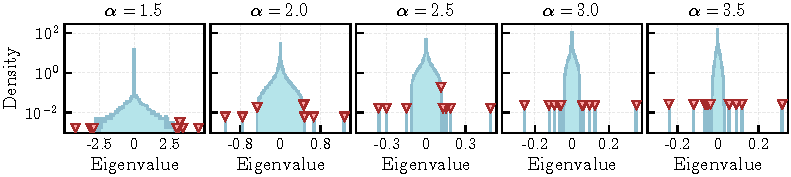
\includegraphics[width=\linewidth]{figs/rf1spec_4panel}
    \caption{
    \textbf{Spectral emergence in the Neural LoFi estimator.}
    Spectrum of the first random-feature spectral operator $\widehat C_1$ for the hierarchical  solvable model of section \ref{sec:the model}, shown at increasing sample exponents $\alpha=\log(n)/\log(d)$. 
    Blue histograms display the bulk eigenvalue density, while red triangles indicate the leading $d_1$ eigenvalues in absolute value. 
    As $\alpha$ increases, the leading eigenvalues progressively separate from the bulk, marking the {\it emergence} of concepts in the first layer, as predicted by the sample-complexity scale $n\gg d^{2+\epsilon}$ (from Eq.~\eqref{eq:lofi-emergence-threshold}) in the quadratic setting $k=2$.
    }
    \label{fig:rf_spectrum}
\end{figure}






Figure~\ref{fig:rf_spectrum} gives a more direct spectral view of the same phenomenon. At small sample sizes, the leading eigenvalues of $\widehat C_1$ remain buried in the random-feature bulk. As $\alpha$ increases, the leading $d_1$ eigenvalues separate from the bulk and become stable outliers. This outlier formation is the spectral signature of the first-layer signal emerging in the random-feature representation. Together with the overlap curve, it shows that Neural LoFi recovers the hidden degree-$2$ representation at the same sample scale predicted by the Hermite theory, while avoiding the explicit construction of the Hermite feature map.
